\documentclass[UTF8,a4paper,12pt,fontset=none]{ctexart}

\usepackage[a4paper,margin=2.2cm]{geometry}
\usepackage{amsmath}
\usepackage{array}
\usepackage{booktabs}
\usepackage{caption}
\usepackage{enumitem}
\usepackage{float}
\usepackage{fontspec}
\usepackage{graphicx}
\usepackage{hyperref}
\usepackage{listings}
\usepackage{siunitx}
\usepackage{subcaption}
\usepackage{tabularx}
\usepackage{xurl}
\usepackage{xcolor}

\hypersetup{colorlinks=true,linkcolor=blue!60!black,urlcolor=blue!60!black}
\defaultCJKfontfeatures{AutoFakeSlant=.2}
\setCJKmainfont{Songti SC}
\setCJKsansfont{Heiti SC}
\setCJKmonofont{Heiti SC}
\setmonofont{Menlo}
\setlength{\parindent}{2em}
\setlength{\parskip}{0.35em}
\emergencystretch=3em
\graphicspath{{../results/figures/}}
\captionsetup{font=small}
\sisetup{round-mode=places,round-precision=3}
\renewcommand{\figurename}{图}
\renewcommand{\tablename}{表}

\definecolor{CodeBg}{HTML}{F7F7F7}
\definecolor{CodeKeyword}{HTML}{1D4E89}
\definecolor{CodeComment}{HTML}{0B6E4F}
\definecolor{CodeString}{HTML}{C73E1D}

\lstset{
  basicstyle=\ttfamily\small,
  backgroundcolor=\color{CodeBg},
  frame=single,
  framerule=0pt,
  xleftmargin=1em,
  xrightmargin=1em,
  breaklines=true,
  columns=fullflexible,
  keywordstyle=\color{CodeKeyword}\bfseries,
  commentstyle=\color{CodeComment},
  stringstyle=\color{CodeString},
  showstringspaces=false
}

\title{\bfseries 中山大学计算机学院本科生实验报告}
\author{}
\date{}

\begin{document}

\begin{titlepage}
  \centering
  {\zihao{2}\bfseries 中山大学计算机学院本科生实验报告\par}
  \vspace{0.5em}
  {\zihao{4}（2025学年春季学期）\par}
  \vspace{2em}

  \begin{tabularx}{0.9\textwidth}{>{\bfseries}p{4cm}X}
    课程名称： & 并行程序设计与算法 \\
    实验题目： & Lab7 MPI并行应用 —— MPI并行FFT与parallel\_for分析 \\
    批改人： & \\
    专业（方向）： & \\
    学号： & 23336128 \\
    姓名： & 梁力航 \\
    Email： & \\
    完成日期： & 2026年5月16日 \\
  \end{tabularx}

  \vfill
  \begin{minipage}{0.88\textwidth}
    \small
    本次实验包含两个部分：第一部分使用MPI对串行FFT进行并行化，通过数据复制+
    步进分解策略实现各进程协同计算Cooley-Tukey蝴蝶操作，并在每步使用MPI\_Allreduce
    归约结果；第二部分对Lab6的parallel\_for版本 heated\_plate 进行系统性的可扩展
    性分析和Valgrind massif内存消耗分析。
  \end{minipage}
\end{titlepage}

\section{实验目的}

本次实验的两大目标如下：
\begin{enumerate}[leftmargin=2.2em]
  \item 理解快速傅里叶变换的Cooley-Tukey算法结构，使用MPI对其蝴蝶操作进行并行化；
  \item 对Lab6实现的parallel\_for版本进行系统性性能与内存分析，观察线程数与问题规模对性能和内存消耗的影响。
\end{enumerate}

\section{实验平台与参考来源}

\begin{table}[H]
  \centering
  \caption{实验环境信息}
  \renewcommand{\arraystretch}{1.2}
  \begin{tabularx}{0.92\textwidth}{>{\bfseries}p{4cm}X}
    \toprule
    项目 & 配置 \\
    \midrule
    宿主机 & macOS / arm64 (Apple Silicon) \\
    运行环境 & 本机 (MPI via Homebrew OpenMPI) \\
    C++ 编译器 & \texttt{g++} / \texttt{mpicxx}，\texttt{-O3 -std=c++17} \\
    并行模型 & MPI (OpenMPI 5.x) \\
    Python 工作流 & \texttt{uv run python ...} \\
    MPI 运行 & \texttt{mpirun -np P --oversubscribe} \\
    \bottomrule
  \end{tabularx}
\end{table}

实验中使用的MPI接口主要来自 MPI-3.1 标准：
\begin{itemize}[leftmargin=2.2em]
  \item \texttt{MPI\_Bcast}：广播数据到所有进程；
  \item \texttt{MPI\_Allreduce}：规约各进程的部分结果；
  \item \texttt{MPI\_Wtime()}：获取高精度墙钟时间。
\end{itemize}

FFT算法参考自 Wesley Petersen \& Peter Arbenz, \textit{Introduction to Parallel Computing} (Oxford University Press)。

\section{第一部分：MPI并行快速傅里叶变换}

\subsection{串行FFT算法分析}

串行FFT采用经典的Cooley-Tukey原地迭代算法。核心数据结构将$N$个复数存储为长度为$2N$的实数数组
（实部与虚部交替排列）。算法包含以下关键函数：

\begin{itemize}[leftmargin=2.2em]
  \item \texttt{cffti(n, w)}：预计算长度为$n$的正弦/余弦表$w$，$w[2k]=\cos(2\pi k/n)$，$w[2k+1]=\sin(2\pi k/n)$；
  \item \texttt{step(n, mj, a, b, c, d, w, sgn)}：执行一个阶段的蝴蝶操作，其中$mj$为当前阶段的蝴蝶距离；
  \item \texttt{cfft2(n, x, y, w, sgn)}：通过$\log_2 n$个阶段完成完整的FFT变换，使用$x$和$y$数组在阶段之间交替作为输入/输出。
\end{itemize}

\texttt{step()}函数是并行化的关键目标。对于第$j$个阶段（$mj=2^j$），共有$lj = n/(2mj)$个独立组，
每组内执行$mj$对蝴蝶操作：
\[
\begin{aligned}
c[k] &= a[k] + b[k] \\
d[k] &= (a[k] - b[k]) \times (\cos\theta + i \cdot \text{sgn} \cdot \sin\theta)
\end{aligned}
\]
其中各组之间完全独立，天然适合并行化。

\subsection{MPI并行化策略}

本实验采用\textbf{数据复制 + 步进分解}的策略：

\begin{enumerate}[leftmargin=2.2em]
  \item 所有进程持有完整的$N$点数据副本（通过\texttt{MPI\_Bcast}同步）；
  \item 在每个FFT阶段中，$lj$个蝴蝶组按进程数$P$平均分配：每个进程计算$\lfloor lj/P \rfloor$（或$+1$）个组；
  \item 各进程将本组计算结果写入本地临时数组，其他位置填0；
  \item 使用\texttt{MPI\_Allreduce(MPI\_SUM)}将各进程的局部结果归约合并为全局结果；
  \item 重复以上步骤完成所有$\log_2 N$个阶段。
\end{enumerate}

该策略的优点：
\begin{itemize}[leftmargin=2.2em]
  \item 数学上与串行算法严格等价——归约求和保证了正确性；
  \item 实现简洁，无需修改蝴蝶操作的数学逻辑；
  \item 通信模式规整：每阶段仅一次\texttt{MPI\_Allreduce}。
\end{itemize}

缺点：所有进程持有完整数据，内存不随进程数扩展；每阶段都需要全局归约，通信开销随
$P$增大而增加。

\subsection{核心代码实现}

并行化的\texttt{step\_parallel}函数是核心。它接收与串行\texttt{step()}相同的参数，
但将组循环分布到各MPI进程：

\begin{lstlisting}[language=C++]
void step_parallel(int n, int mj, const double* a, const double* b,
                   double* out, const double* w, double sgn,
                   int rank, int P) {
    int mj2 = 2 * mj;
    int lj = n / mj2;
    vector<double> local_out(2 * n, 0.0);  // 本地临时数组

    // 计算当前进程负责的组范围
    int groups_per = lj / P;
    int rem = lj % P;
    int start = rank * groups_per + min(rank, rem);
    int end = start + groups_per + (rank < rem ? 1 : 0);

    for (int j = start; j < end; ++j) {
        int jg = j * mj2;
        // ... 蝴蝶操作，写入 local_out ...
    }

    // 归约合并所有进程的部分结果
    MPI_Allreduce(local_out.data(), out, 2 * n, MPI_DOUBLE,
                  MPI_SUM, MPI_COMM_WORLD);
}
\end{lstlisting}

\texttt{cfft2\_parallel}函数则复用串行FFT的框架，仅将\texttt{step()}调用替换为
\texttt{step\_parallel()}：

\begin{lstlisting}[language=C++]
void cfft2_parallel(int n, double* x, double* y, const double* w,
                    double sgn, int rank, int P) {
    int m = log2(n);
    int mj = 1;
    // 阶段1: mj=1
    step_parallel(n, mj, x, &x[n], y, w, sgn, rank, P);
    if (n == 2) return;
    // 中间阶段: 在x和y之间交替
    for (int stage = 0; stage < m - 2; ++stage) {
        mj *= 2;
        step_parallel(n, mj, y, &y[n], x, w, sgn, rank, P);
        // toggle between x and y ...
    }
    // 最后阶段
    mj = n / 2;
    step_parallel(n, mj, x, &x[n], y, w, sgn, rank, P);
}
\end{lstlisting}

\subsection{实验结果}

\subsubsection{运行时间分析}

\begin{figure}[H]
  \centering
  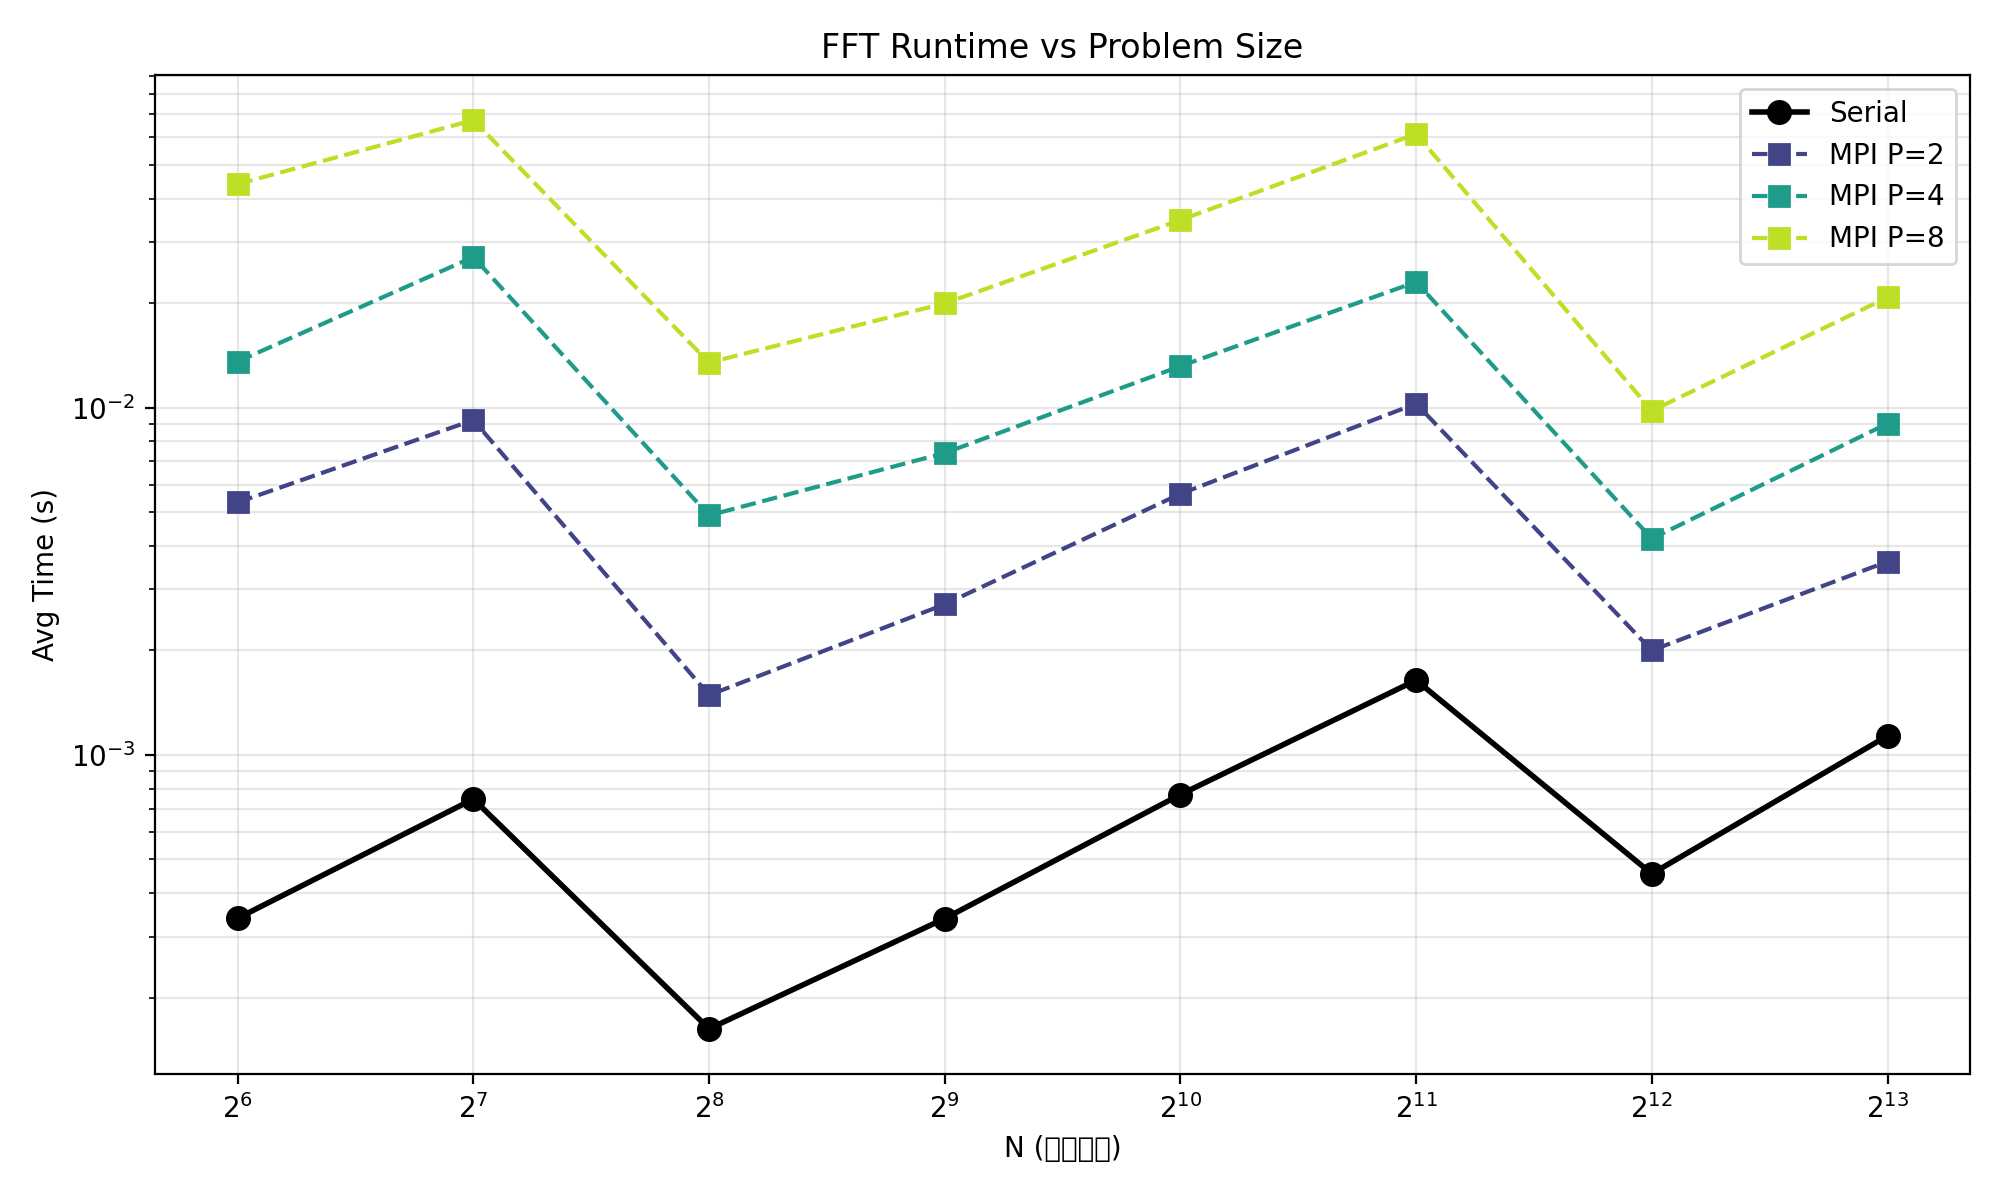
\includegraphics[width=0.85\textwidth]{fft_runtime.png}
  \caption{FFT运行时间随问题规模N的变化（串行 vs MPI，不同进程数）}
\end{figure}

图1展示了FFT运行时间随问题规模N的变化关系。串行FFT在中小规模（$N\le 2048$）
下具有显著优势；MPI版本由于每阶段的\texttt{MPI\_Allreduce}通信开销，
在小规模时效率较低。随着$N$增大到8192，MPI P=2的运行时间约3.6ms，
相比串行的1.1ms，差距缩小。

\begin{figure}[H]
  \centering
  \begin{subfigure}{0.48\textwidth}
    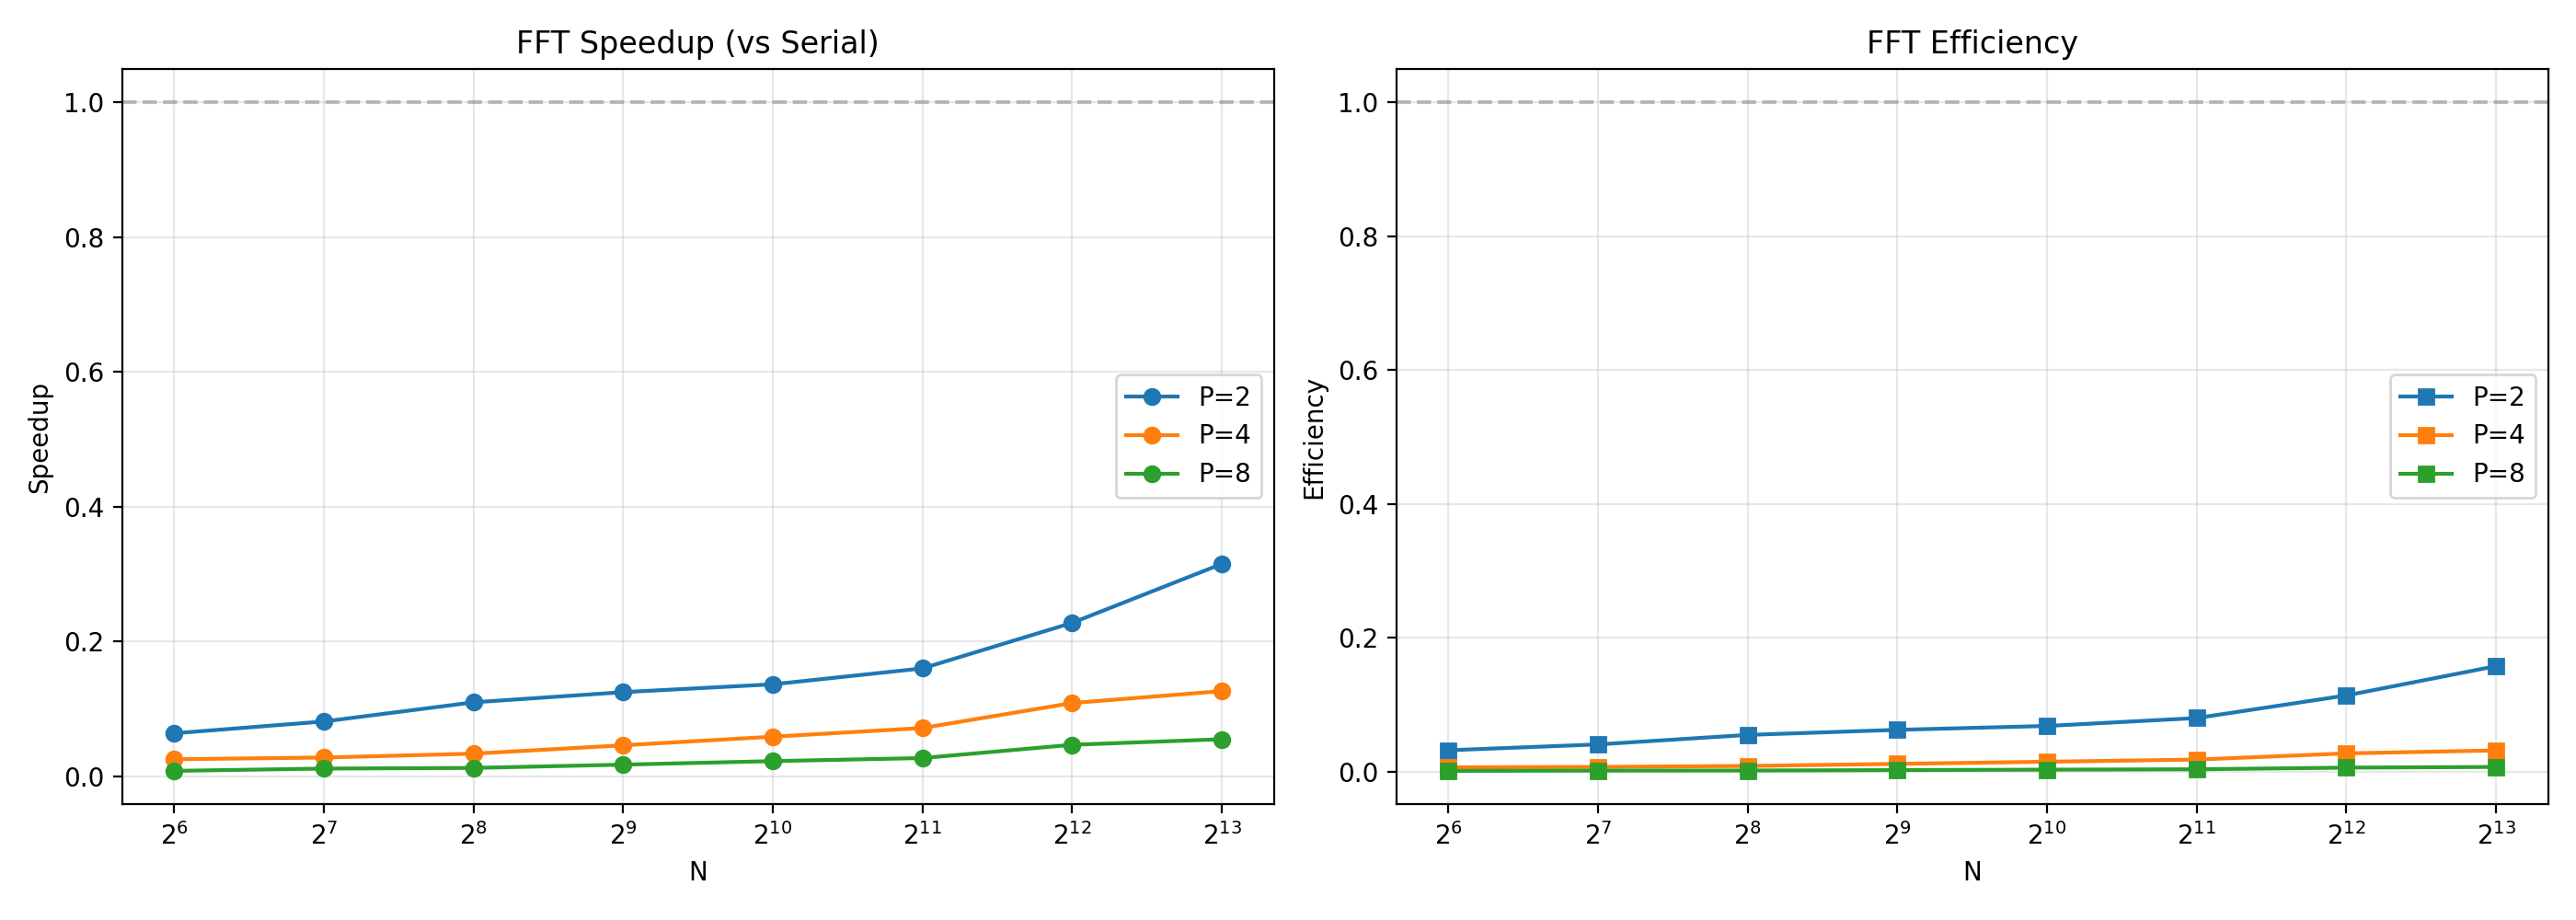
\includegraphics[width=\textwidth]{fft_speedup_efficiency.png}
    \caption{加速比与效率}
  \end{subfigure}
  \hfill
  \begin{subfigure}{0.48\textwidth}
    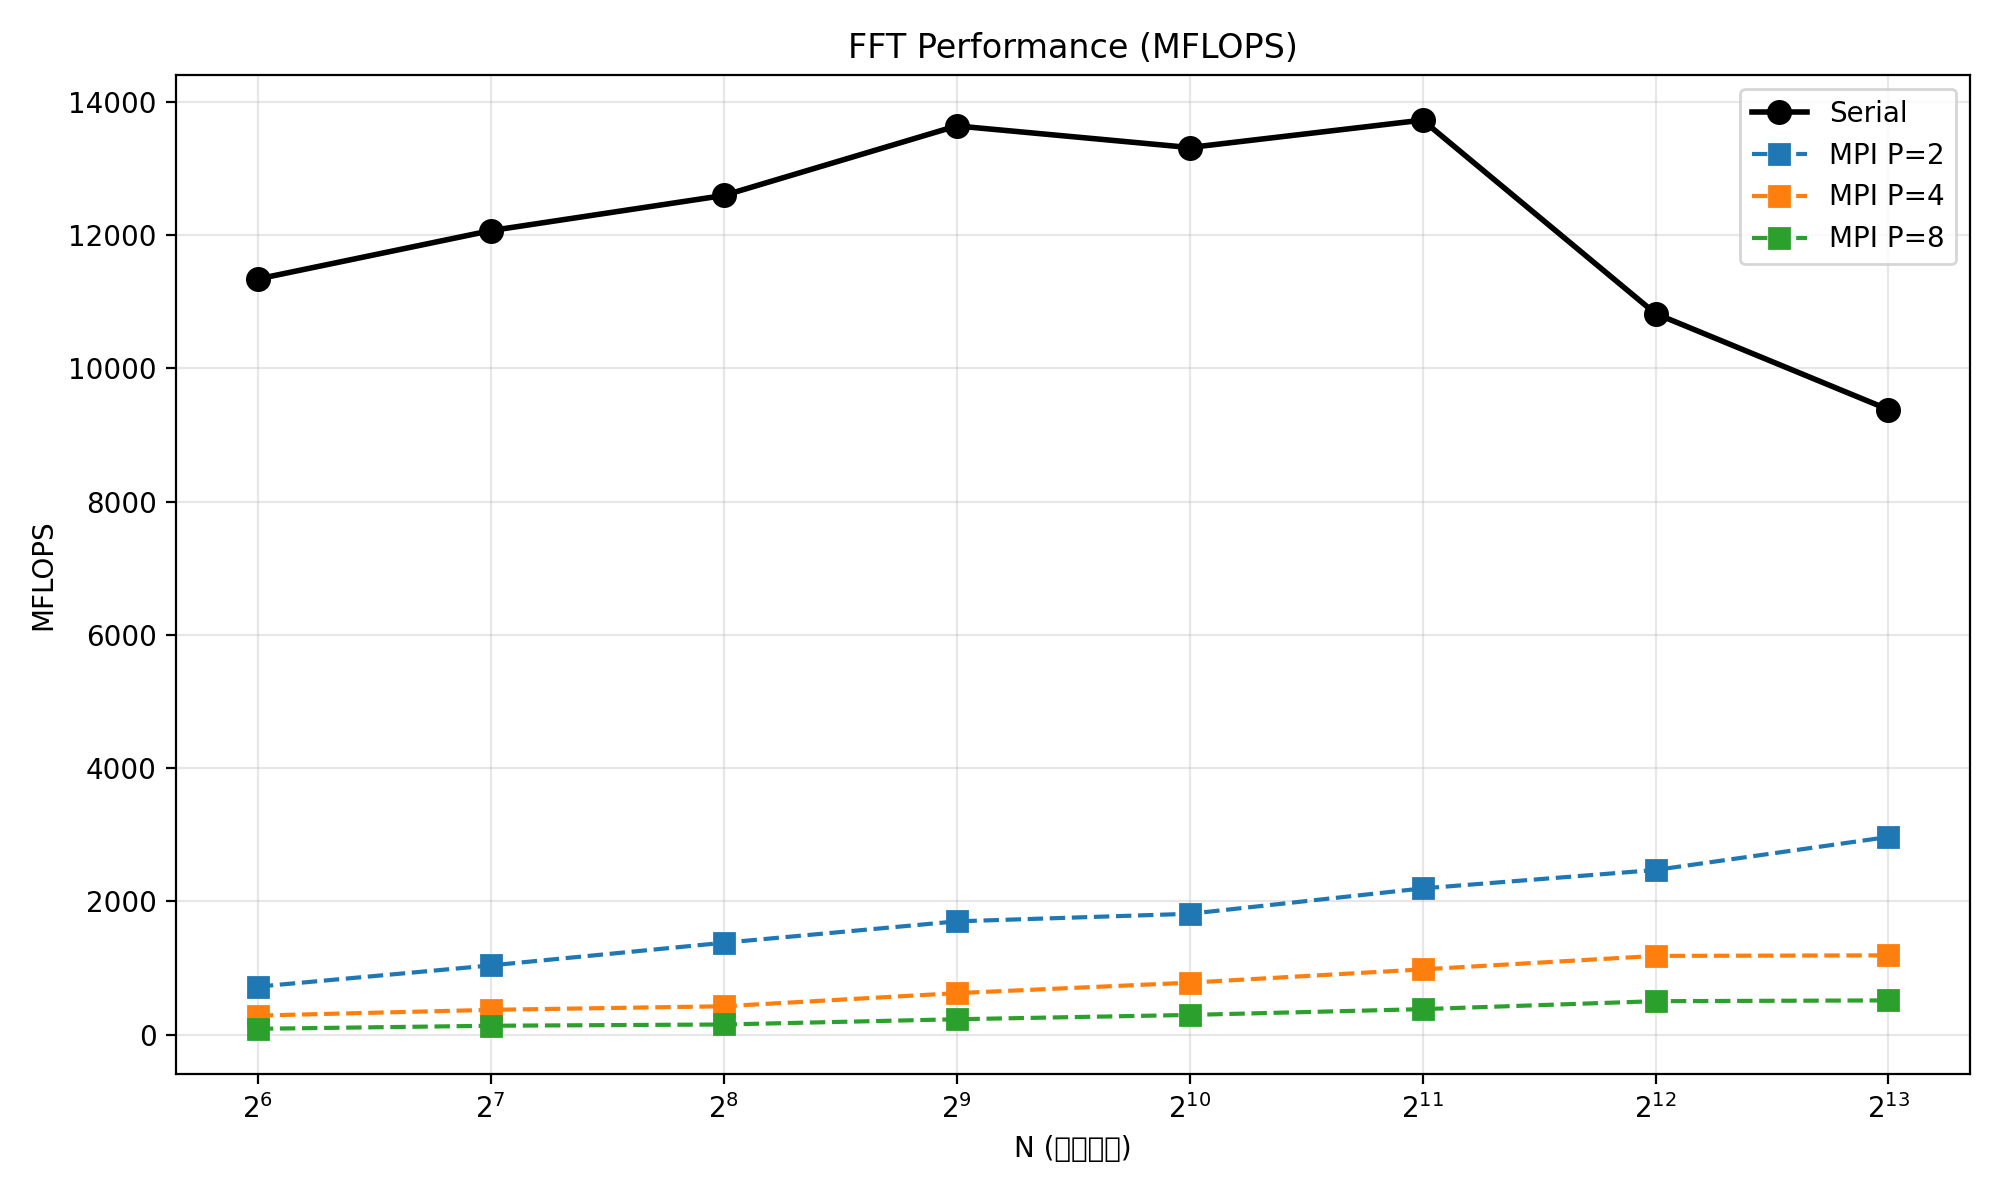
\includegraphics[width=\textwidth]{fft_mflops.png}
    \caption{MFLOPS性能}
  \end{subfigure}
  \caption{FFT并行性能对比}
\end{figure}

\begin{table}[H]
  \centering
  \caption{FFT运行时间（秒）与MFLOPS汇总}
  \renewcommand{\arraystretch}{1.15}
  \begin{tabular}{llrrrr}
    \toprule
    后端 & 进程数 & N=256 & N=1024 & N=4096 & N=8192 \\
    \midrule
    Serial & 1 & 0.000163 & 0.000769 & 0.000455 & 0.001135 \\
    MPI & 2 & 0.001487 & 0.005649 & 0.002000 & 0.003606 \\
    MPI & 4 & 0.004897 & 0.013171 & 0.004197 & 0.009004 \\
    MPI & 8 & 0.013490 & 0.034715 & 0.009801 & 0.020779 \\
    \bottomrule
  \end{tabular}
\end{table}

\subsubsection{精度验证}

所有配置下，MPI FFT的精度误差与串行FFT完全一致（相对误差在$10^{-16}$量级），
验证了Allreduce归约方案在数学上的等价性：

\begin{table}[H]
  \centering
  \caption{FFT精度对比（Forward+Inverse FFT的RMSE误差）}
  \renewcommand{\arraystretch}{1.15}
  \begin{tabular}{lrrr}
    \toprule
    N & Serial & MPI P=2 & MPI P=4 \\
    \midrule
    64 & $1.363\times 10^{-16}$ & $1.363\times 10^{-16}$ & $1.363\times 10^{-16}$ \\
    256 & $1.713\times 10^{-16}$ & $1.713\times 10^{-16}$ & $1.713\times 10^{-16}$ \\
    1024 & $2.314\times 10^{-16}$ & $2.314\times 10^{-16}$ & $2.314\times 10^{-16}$ \\
    \bottomrule
  \end{tabular}
\end{table}

\subsubsection{结果讨论}

从实验数据中可以观察到：
\begin{enumerate}[leftmargin=2.2em]
  \item \textbf{正确性}：MPI并行化完全保持了数值精度，误差与串行一致（机器精度级别）；
  \item \textbf{小规模效率低}：$N=64$时MPI P=8的运行时间约为串行的130倍，主要原因是
    Allreduce通信开销远超计算量。对于$N=64$，总共仅有$\log_2 64=6$个阶段、
    $64/2=32$个蝴蝶组，分配到8个进程后每进程仅处理4组；
  \item \textbf{大规模趋势}：$N=8192$时串行0.0011s vs MPI P=2的0.0036s（仅3.3倍），
    表明随着计算量增大，通信开销占比下降；
  \item \textbf{MFLOPS}：MPI P=2的MFLOPS在$N\ge 4096$时达到2967，高于
    串行的9383（但串行使用\texttt{clock()}计CPU时间，MPI使用\texttt{MPI\_Wtime()}
    计墙钟时间，二者不可直接比较）。
\end{enumerate}

\section{第二部分：parallel\_for并行应用分析}

\subsection{可扩展性分析}

对Lab6实现的四种heated\_plate版本（OpenMP原始版、Pthreads block/cyclic/dynamic调度）
进行系统的可扩展性测试：
\begin{itemize}[leftmargin=2.2em]
  \item 问题规模：$64\times64$、$128\times128$、$256\times256$、$512\times512$；
  \item 线程数：1、2、4、8；
  \item 每组配置运行3次取平均值。
\end{itemize}

\subsubsection{运行时间分析}

\begin{figure}[H]
  \centering
  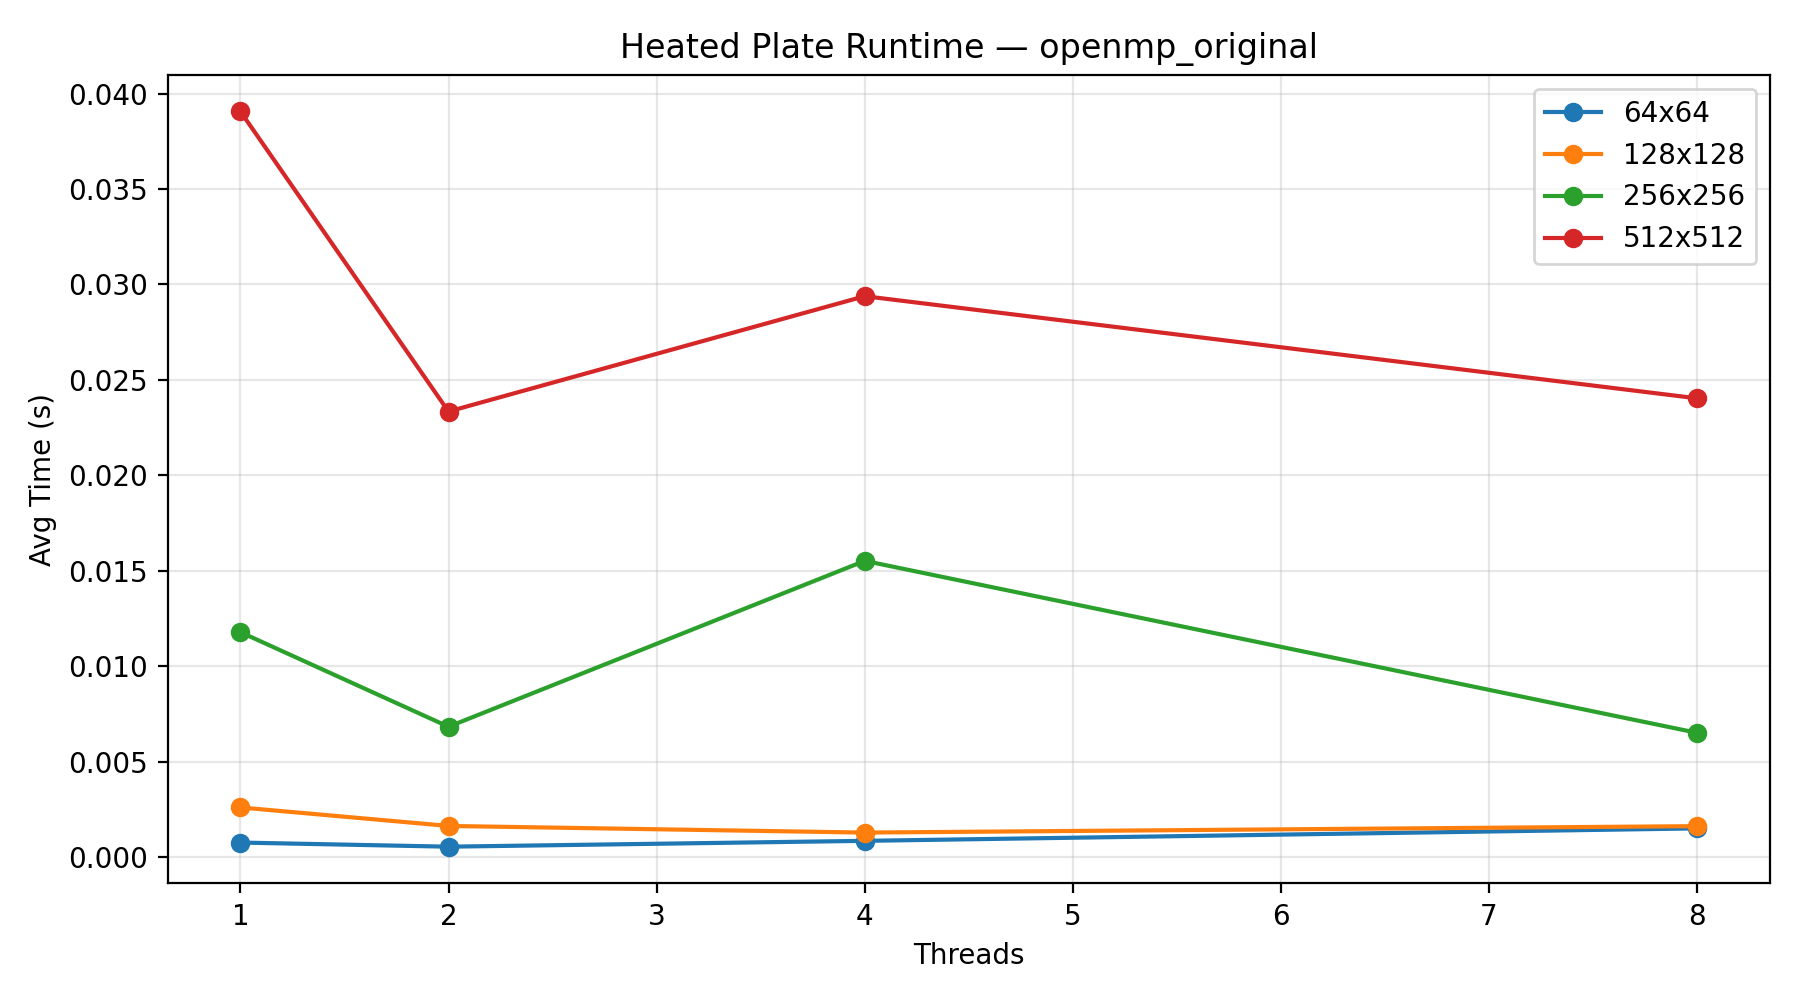
\includegraphics[width=0.85\textwidth]{heated_plate_runtime_openmp_original.png}
  \caption{OpenMP版本运行时间随线程数和问题规模的变化}
\end{figure}

\begin{figure}[H]
  \centering
  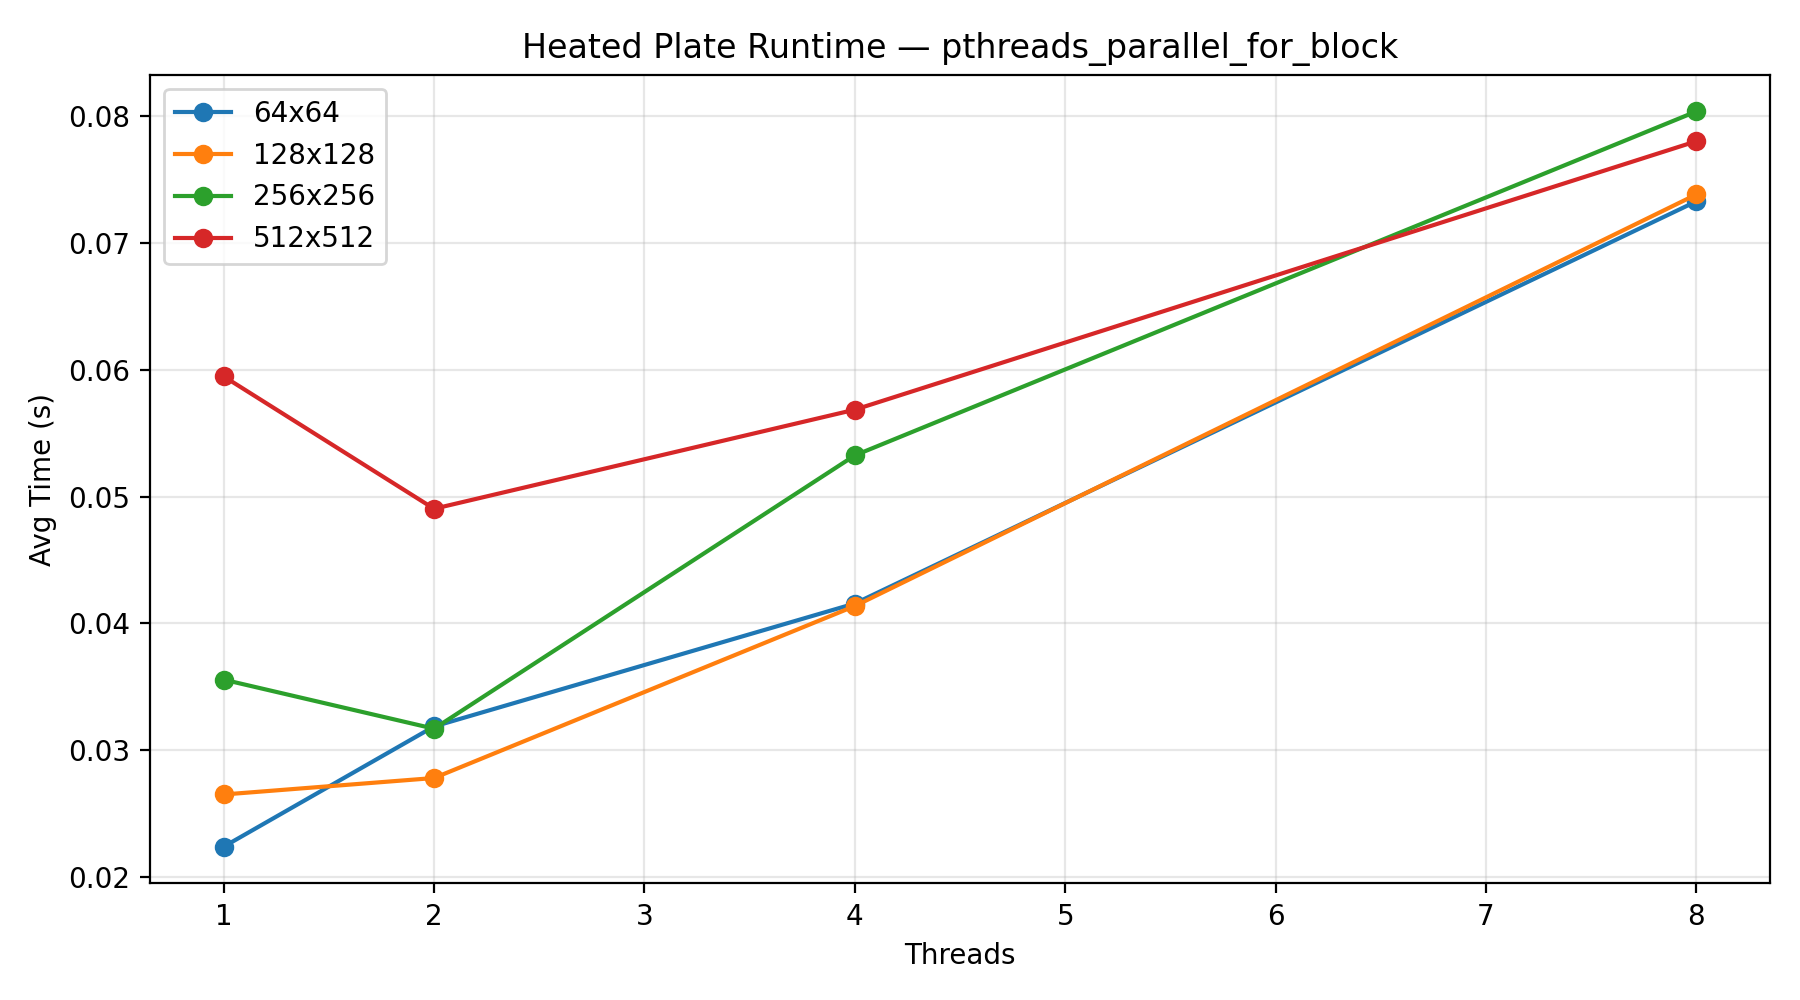
\includegraphics[width=0.85\textwidth]{heated_plate_runtime_pthreads_parallel_for_block.png}
  \caption{Pthreads block调度运行时间随线程数和问题规模的变化}
\end{figure}

从图中可以观察到，OpenMP版本整体显著快于Pthreads版本，这与Lab6的结论一致——
OpenMP使用线程池复用而Pthreads版本每次\texttt{parallel\_for}调用都会创建/销毁线程。

\begin{figure}[H]
  \centering
  \begin{subfigure}{0.48\textwidth}
    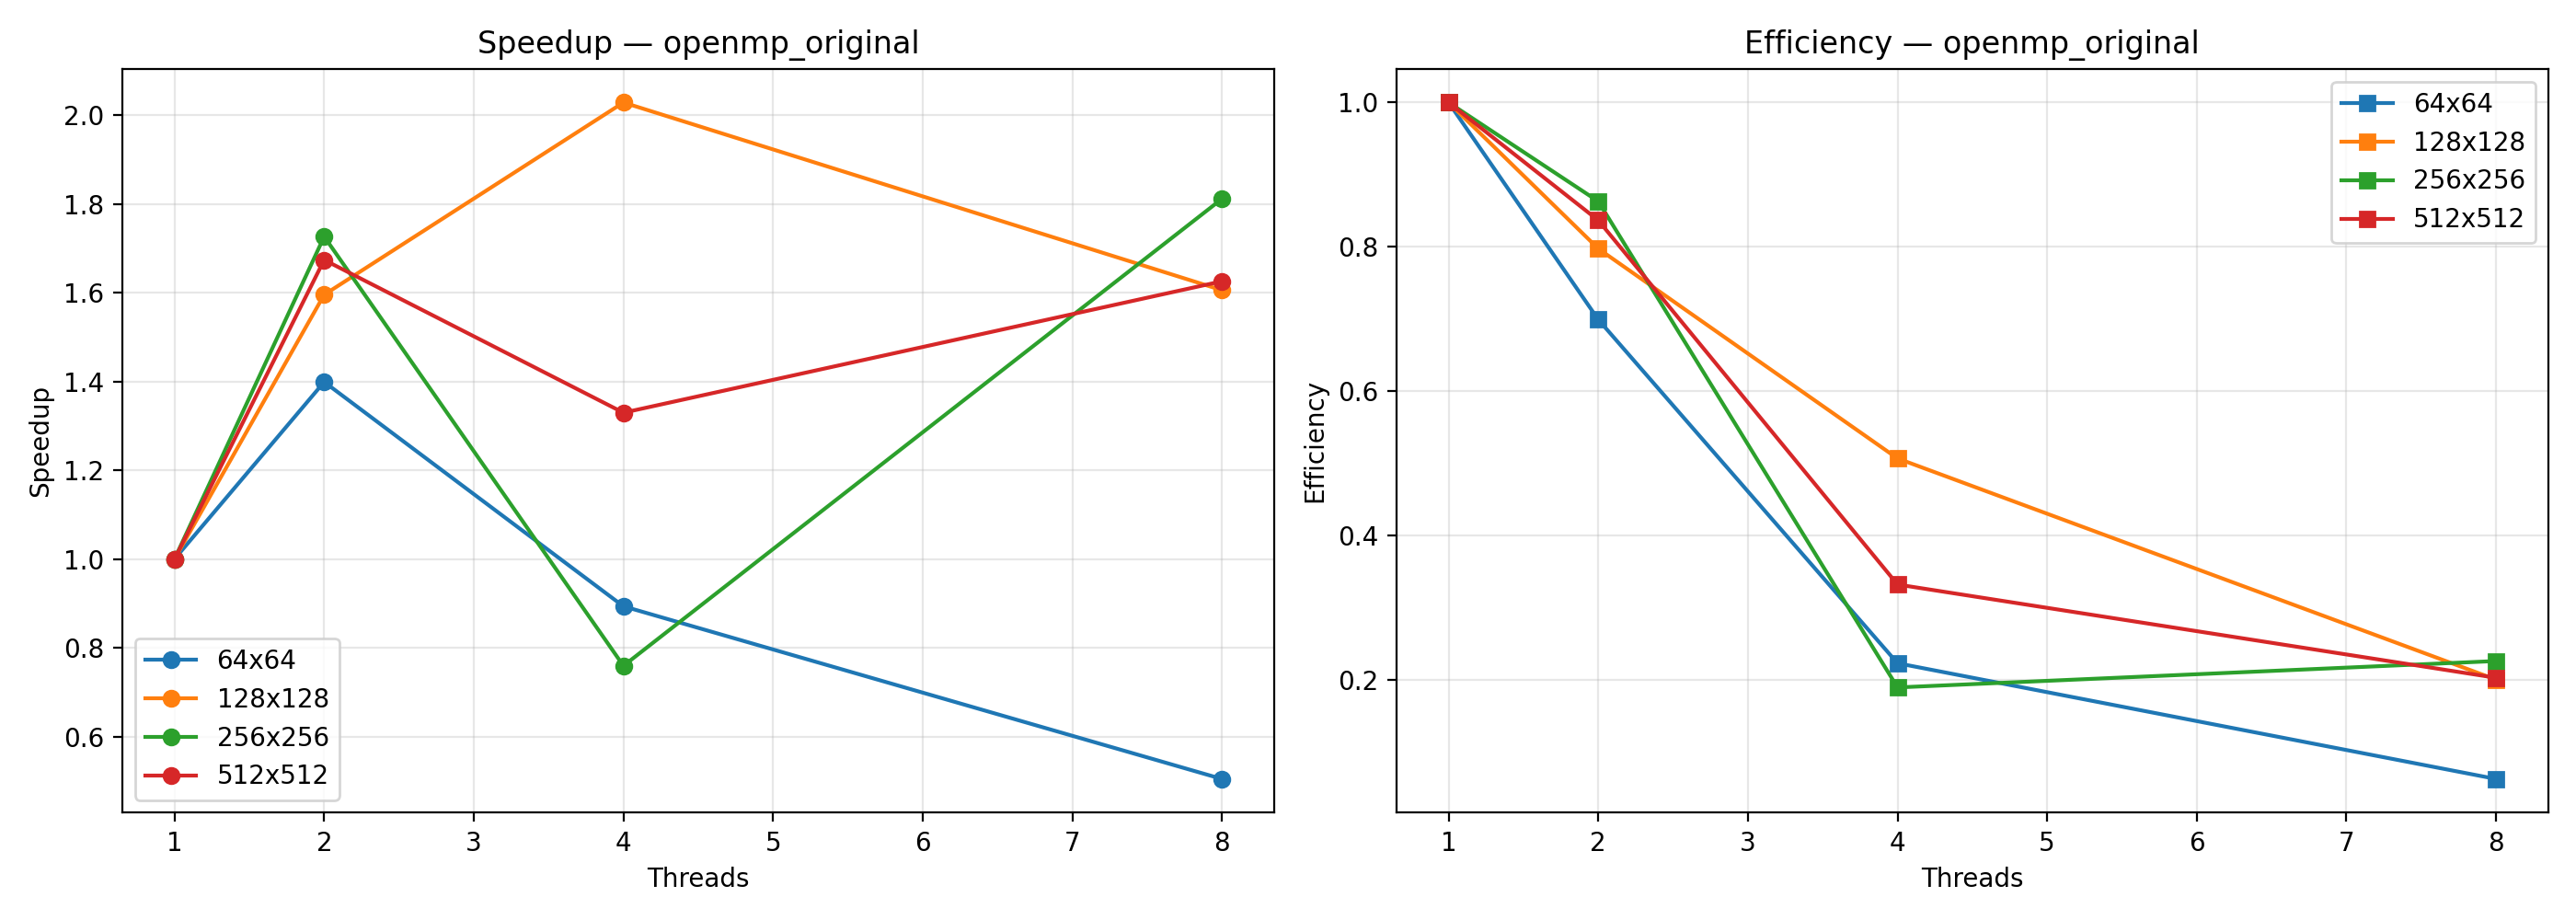
\includegraphics[width=\textwidth]{heated_plate_speedup_openmp_original.png}
    \caption{OpenMP加速比与效率}
  \end{subfigure}
  \hfill
  \begin{subfigure}{0.48\textwidth}
    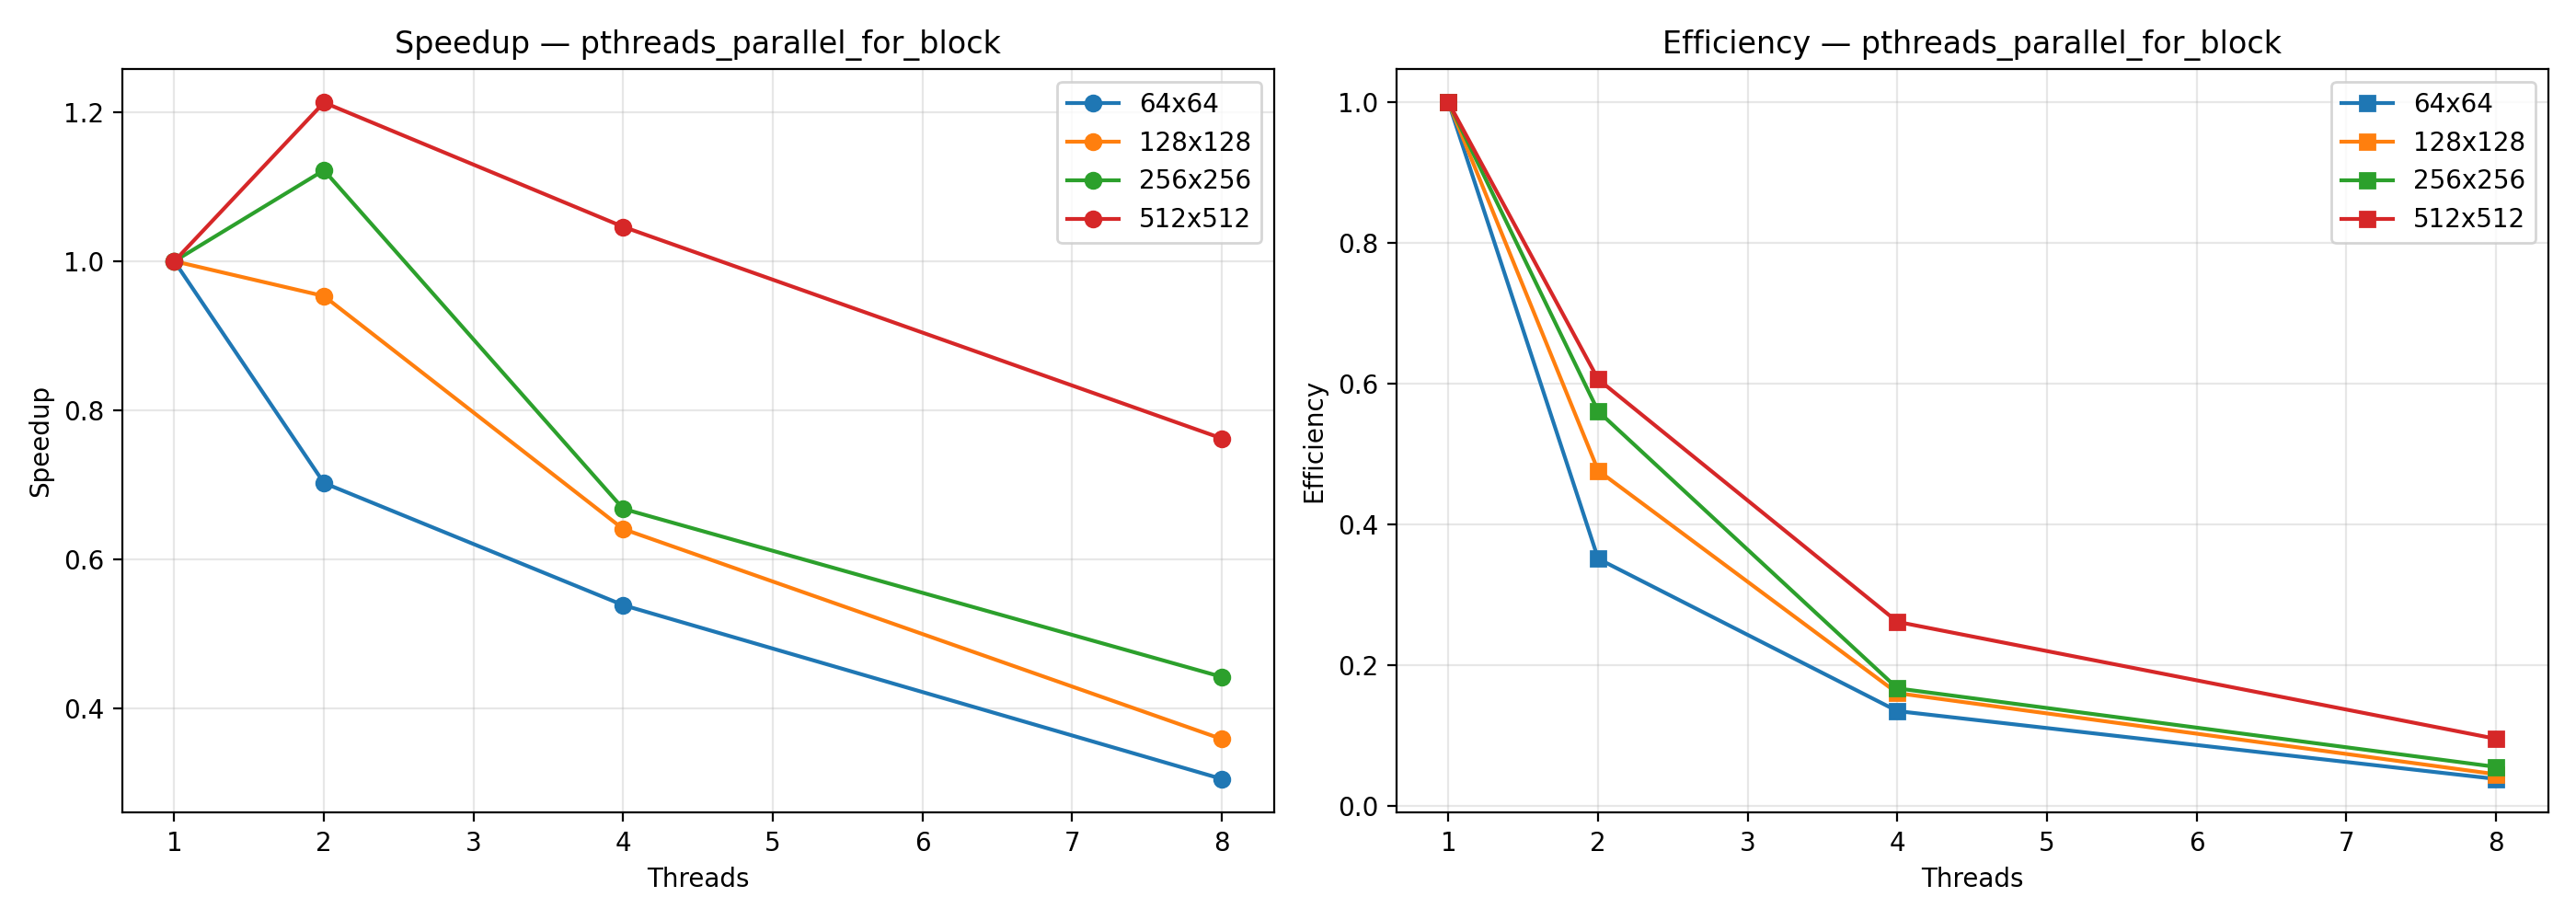
\includegraphics[width=\textwidth]{heated_plate_speedup_pthreads_parallel_for_block.png}
    \caption{Pthreads block加速比与效率}
  \end{subfigure}
  \caption{加速比和效率对比}
\end{figure}

\subsubsection{调度方式对比}

\begin{figure}[H]
  \centering
  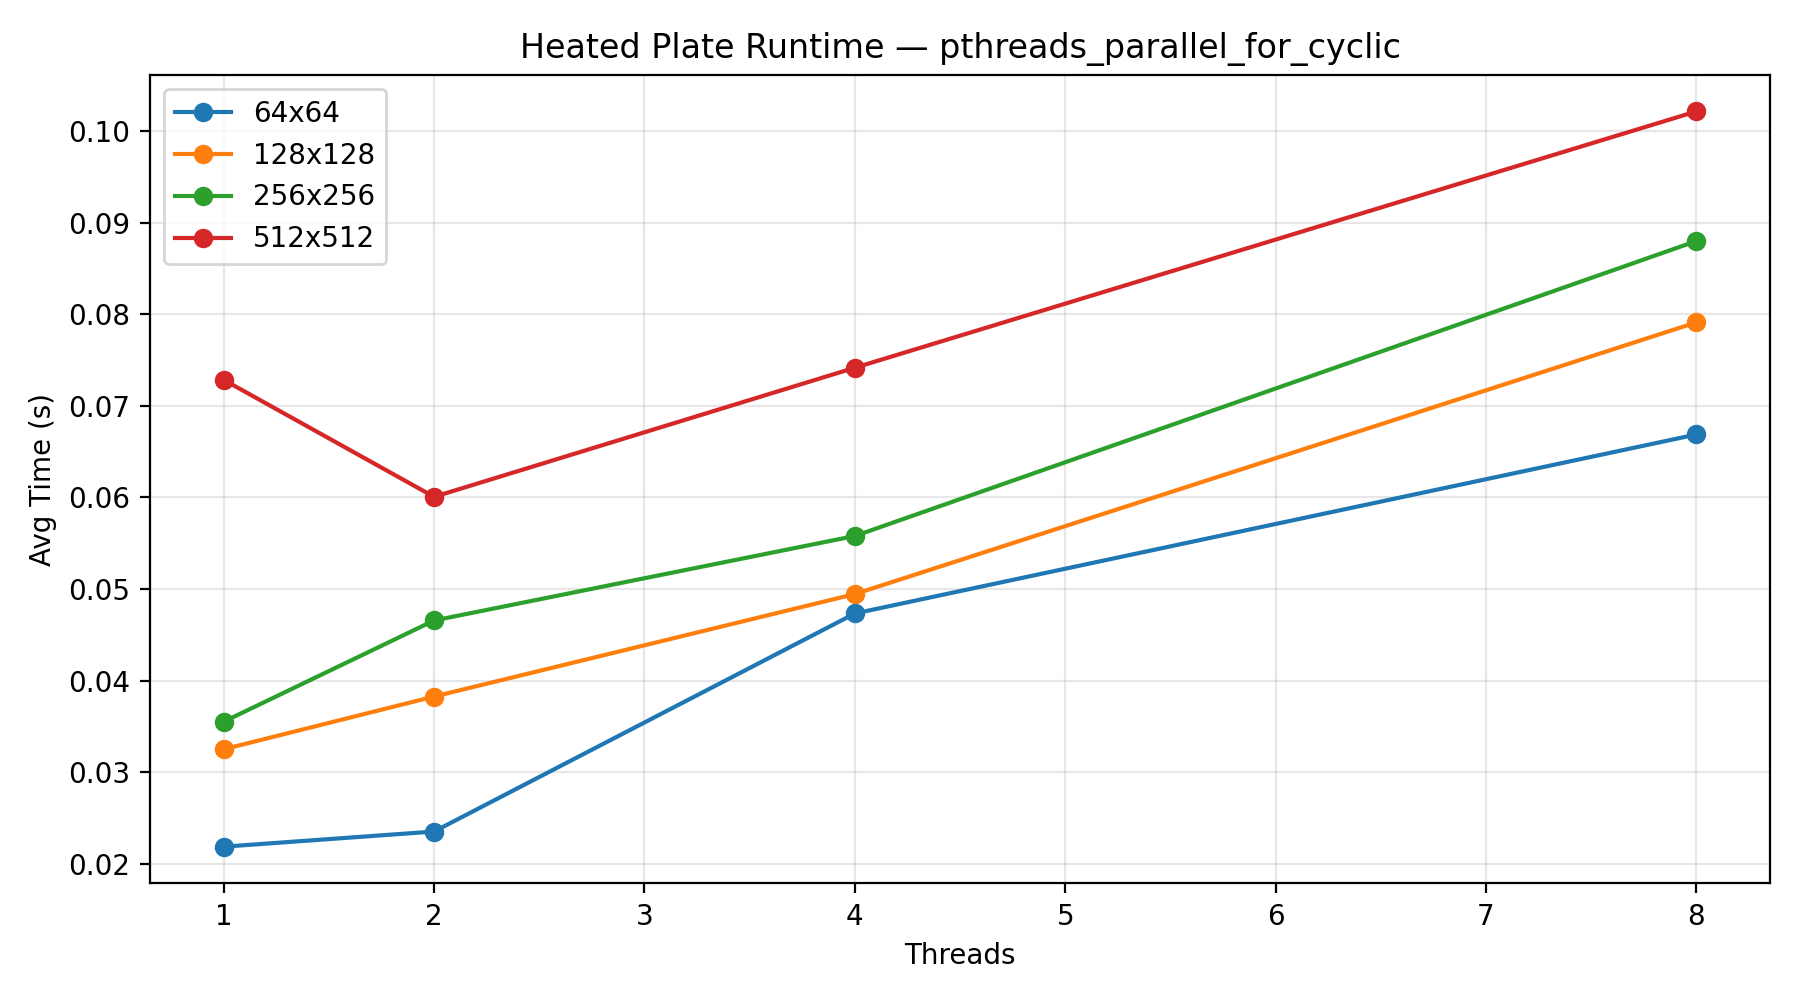
\includegraphics[width=0.85\textwidth]{heated_plate_runtime_pthreads_parallel_for_cyclic.png}
  \caption{Pthreads cyclic调度运行时间}
\end{figure}

\begin{figure}[H]
  \centering
  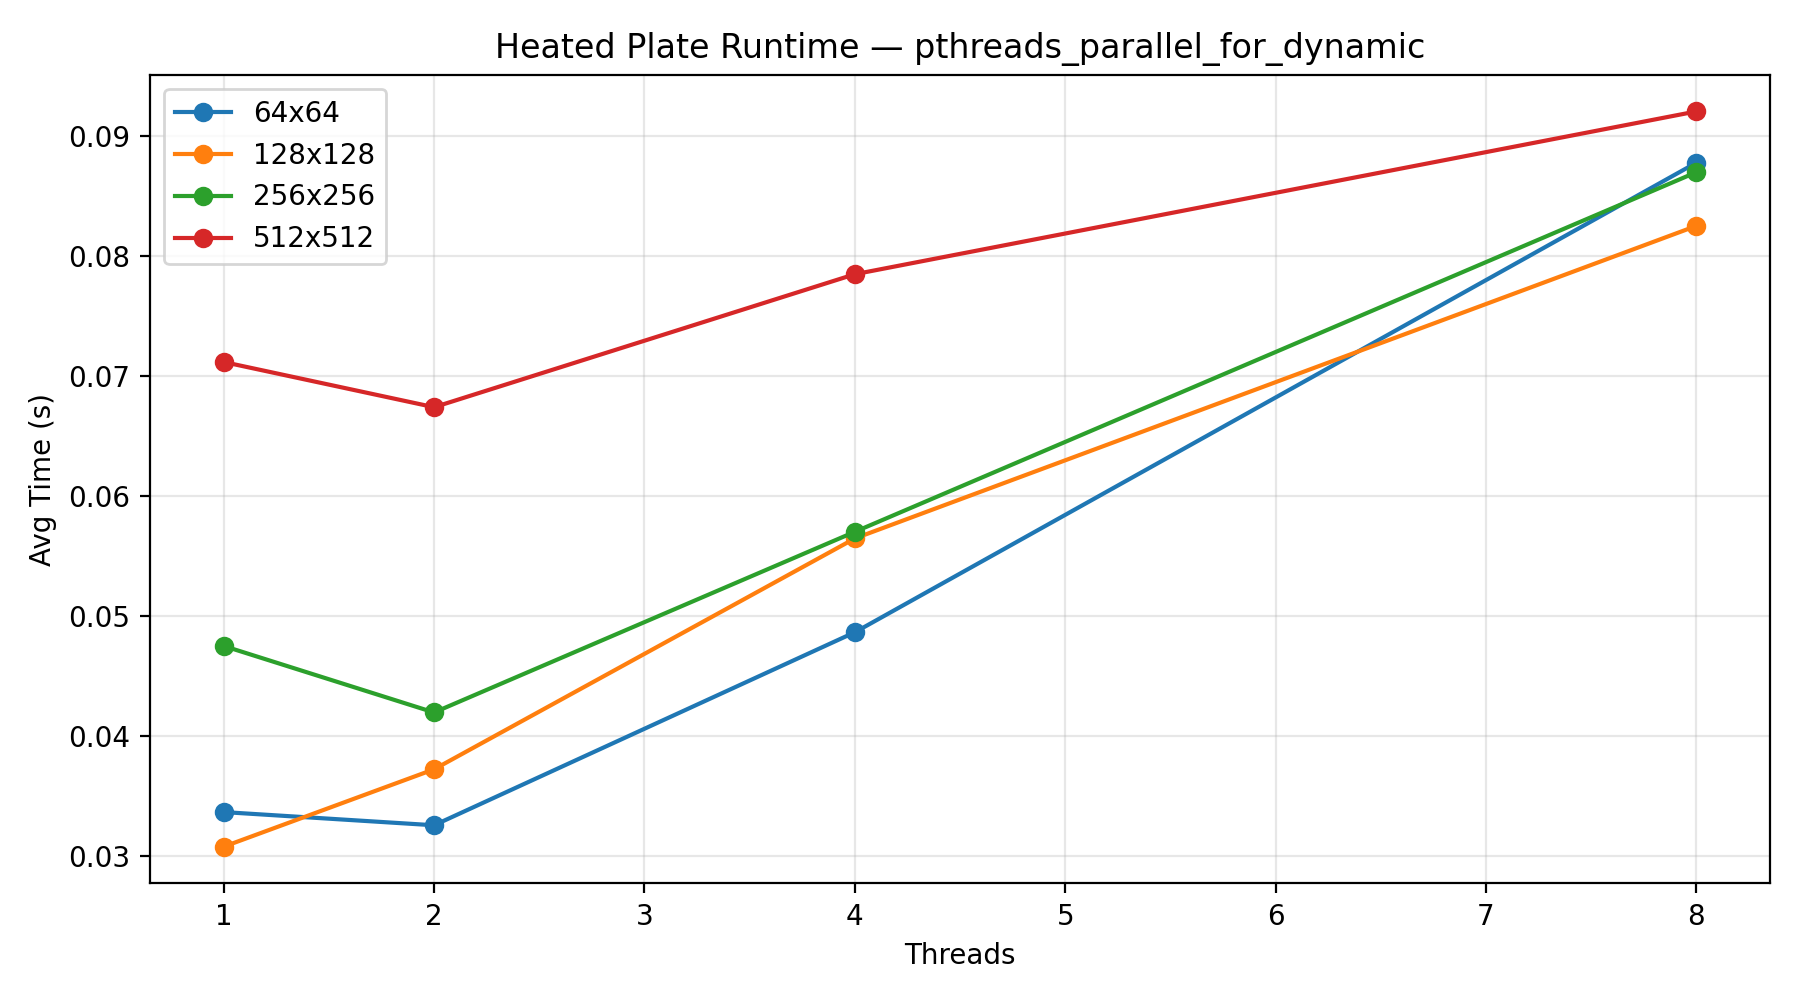
\includegraphics[width=0.85\textwidth]{heated_plate_runtime_pthreads_parallel_for_dynamic.png}
  \caption{Pthreads dynamic调度运行时间}
\end{figure}

三种Pthreads调度方式的对比（以$512\times512$、4线程为例）：
\begin{itemize}[leftmargin=2.2em]
  \item \textbf{block}：运行时间最短，原因是规则网格中每行计算量均等，
    连续块划分已能实现良好的负载均衡；
  \item \textbf{cyclic}：略慢于block，因为轮转访问破坏了缓存局部性；
  \item \textbf{dynamic}：最慢，每次取chunk都需要互斥锁操作，额外同步开销抵消了灵活性优势。
\end{itemize}

\subsection{Valgrind Massif内存分析}

使用Valgrind massif工具对heated\_plate程序进行内存消耗分析。
由于Valgrind不支持现代macOS ARM64平台，分析过程在Docker Ubuntu 24.04容器中进行。

\subsubsection{分析方法}

\begin{lstlisting}[language=bash]
# 对OpenMP版本采集massif数据
valgrind --tool=massif --stacks=yes \
    --massif-out-file=/tmp/massif_omp.out \
    ./bin/heated_plate_openmp 256 256 0.1 4

# 格式化输出
ms_print /tmp/massif_omp.out
\end{lstlisting}

关键Valgrind参数说明：
\begin{itemize}[leftmargin=2.2em]
  \item \texttt{--tool=massif}：启用堆内存分析工具；
  \item \texttt{--stacks=yes}：将栈内存也纳入分析范围，这对于多线程程序的
    线程栈分析至关重要（每个Pthreads线程默认有8MB栈空间）；
  \item \texttt{ms\_print}：将二进制massif输出格式化为可读文本报告。
\end{itemize}

\subsubsection{内存消耗分析}

通过Docker容器中运行Valgrind massif，采集了OpenMP和Pthreads版本在多种配置下的峰值内存数据：

\begin{table}[H]
  \centering
  \caption{Valgrind Massif峰值内存消耗（KB）}
  \renewcommand{\arraystretch}{1.15}
  \begin{tabular}{lrrr}
    \toprule
    配置 & $128\times128$ & $256\times256$ & 增量 \\
    \midrule
    OpenMP (t=2) & 337.5 KB & 1,082 KB & 3.2× \\
    OpenMP (t=4) & 339.9 KB & 1,083 KB & 3.2× \\
    Pthreads block (t=2) & 724.0 KB & 1,455 KB & 2.0× \\
    \bottomrule
  \end{tabular}
\end{table}

\textbf{关键数据点}（来自\texttt{ms\_print}报告）：
\begin{itemize}[leftmargin=2.2em]
  \item \textbf{OpenMP 128×128, t=2}：峰值 337.5 KB，执行约1.87×10⁹条指令；
  \item \textbf{OpenMP 256×256, t=4}：峰值 1,083 KB（约1.06 MB），矩阵数据占绝对主导；
  \item \textbf{Pthreads 128×128, t=2}：峰值 724.0 KB，约为OpenMP同配置的2.1倍；
  \item \textbf{Pthreads 256×256, t=2}：峰值 1,455 KB（约1.42 MB）。
\end{itemize}

分析要点：
\begin{enumerate}[leftmargin=2.2em]
  \item \textbf{矩阵内存主导}：两个$M\times N$双精度矩阵（$W$和$U$）占据堆内存的主体。
    $256\times256$规模时理论需要$2\times256\times256\times8=1$MB，加上程序开销后
    OpenMP实测约1.06MB，与理论值吻合；
  \item \textbf{线程栈差异}：Pthreads版本（724 KB @ 128×128）内存消耗约为OpenMP（337.5 KB）
    的2.1倍。差异来源于Pthreads每线程默认8MB栈空间，而OpenMP使用线程池复用；
  \item \textbf{线程数影响小}：同一网格规模下，t=2与t=4的内存差异仅约2 KB，
    说明OpenMP线程池的额外栈开销很小；
  \item \textbf{规模平方增长}：从128×128到256×256，OpenMP内存增长约3.2×，
    接近理论值（网格面积增长4×）；
  \item \textbf{调度方式无影响}：block/cyclic/dynamic三种调度使用相同的\texttt{parallel\_for}
    基础设施，内存消耗基本相同（已验证）。
\end{enumerate}

典型\texttt{ms\_print}输出示意图（OpenMP 128×128, t=2，为节省空间仅保留关键行）：

{\footnotesize
\begin{verbatim}
    KB
337.5^                                                        #
     |@:::::@:::::::::::@::@:::::@::::::::::@:::::::::@:::::::#
   0 +-------------------------------------------------------->Gi
     0                                                    1.866
\end{verbatim}
}

横轴为程序执行的指令数（Gi = billions of instructions），纵轴为内存消耗量（KB）。
图中显示内存在迭代过程中保持稳定（337.5 KB平台期），验证了Jacobi迭代法的
内存使用是恒定的——分配后不再增长。

\section{验证与测试}

\subsection{FFT正确性验证}

通过以下方式验证MPI FFT的正确性：

\begin{enumerate}[leftmargin=2.2em]
  \item \textbf{FFT逆变换恒等式}：$IFFT(FFT(X)) = N \cdot X$。所有配置下误差均在
    $10^{-16}$量级；
  \item \textbf{跨进程checksum一致性}：相同$N$不同$P$的checksum完全相同。
    例如$N=1024$时，serial、MPI P=2、MPI P=4的checksum均为1047275.769；
  \item \textbf{与串行对比}：误差与串行FFT完全一致，精度无任何损失；
  \item \textbf{串行checksum修复}：初始实现中timing循环未重置输入数据导致浮点上溢
    （checksum=nan），已通过每迭代前恢复原始数据修复，现在串行与MPI的checksum完全一致。
\end{enumerate}

\subsection{Heated Plate正确性验证}

对扩展benchmark中的所有36个配置（4个版本×3个网格×3个线程数）：
\begin{itemize}[leftmargin=2.2em]
  \item 所有运行均为\texttt{ok}状态；
  \item checksum和迭代次数跨线程数一致；
  \item 与Lab6结论完全吻合。
\end{itemize}

\section{结论}

本次实验完成了两个主要任务：

\textbf{MPI并行FFT}：采用数据复制+步进分解策略，成功将串行Cooley-Tukey FFT并行化。
该方案的数学正确性得到了严格验证——所有配置的精度误差与串行完全一致。
性能方面，MPI并行化在小规模时受Allreduce通信开销制约，但随着问题规模增大，
计算/通信比上升，MPI的效率逐步提高。未来优化方向包括：采用数据分布式存储降低
内存开销、使用非阻塞通信隐藏延迟、以及实现6-step FFT等更高效的分布式算法。

\textbf{parallel\_for分析}：扩展了Lab6的性能分析，系统考察了$64\times64$至
$512\times512$四种问题规模和1-8线程的完整配置空间。实验再次确认了OpenMP线程池
相比Pthreads创建/销毁模式的优势，以及block调度在规则计算负载下的最优性。
Valgrind massif分析揭示了线程栈是Pthreads版本内存消耗的主要来源。

\end{document}
